\documentclass{jarticle}
\usepackage[dvipdfmx]{graphicx}
\usepackage[top=20truemm,bottom=20truemm,left=25truemm,right=25truemm]{geometry}
\setlength\intextsep{0pt}
\setlength\textfloatsep{0pt}
\usepackage{here}


\begin{document}

\section*{04/18 課題1}
\begin{flushright}
	情報学研究科複雑系化学専攻\\
	修士1年 児玉高明
\end{flushright}
\subsection*{練習1}
	各挙動を示すrの値を調べるために、以下の様にrを0〜3まで約0.3のステップで変化させたグラフを描画した.
	\begin{figure}[H]
	\centering
  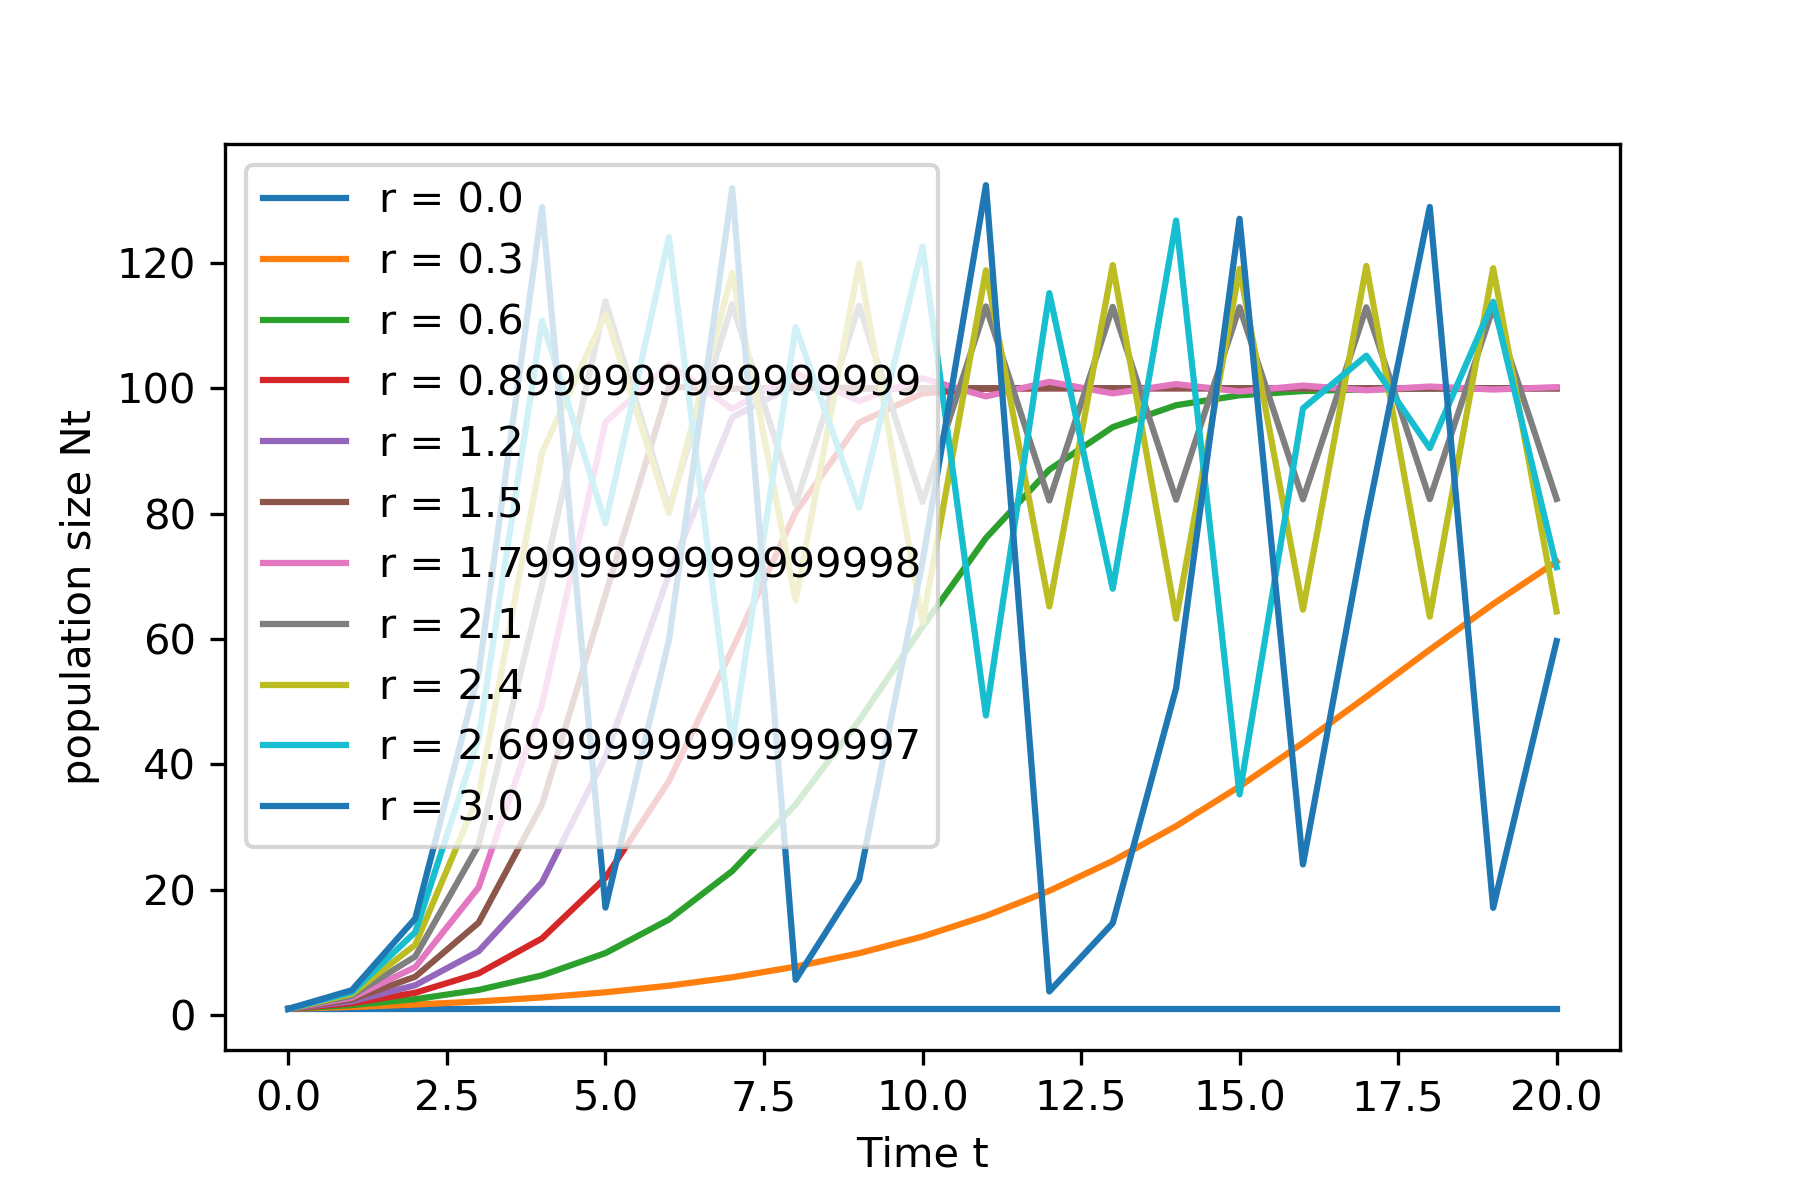
\includegraphics[width=0.8\linewidth]{prep.png}
	\caption{図1 r値による各挙動の推移}
	\end{figure}
	図1より r=0.6, 1.8, 2.7 と選んで, 以下の図2を得た.なお実行したプログラムファイルは0418.pyである.
	\begin{figure}[H]
	\centering
  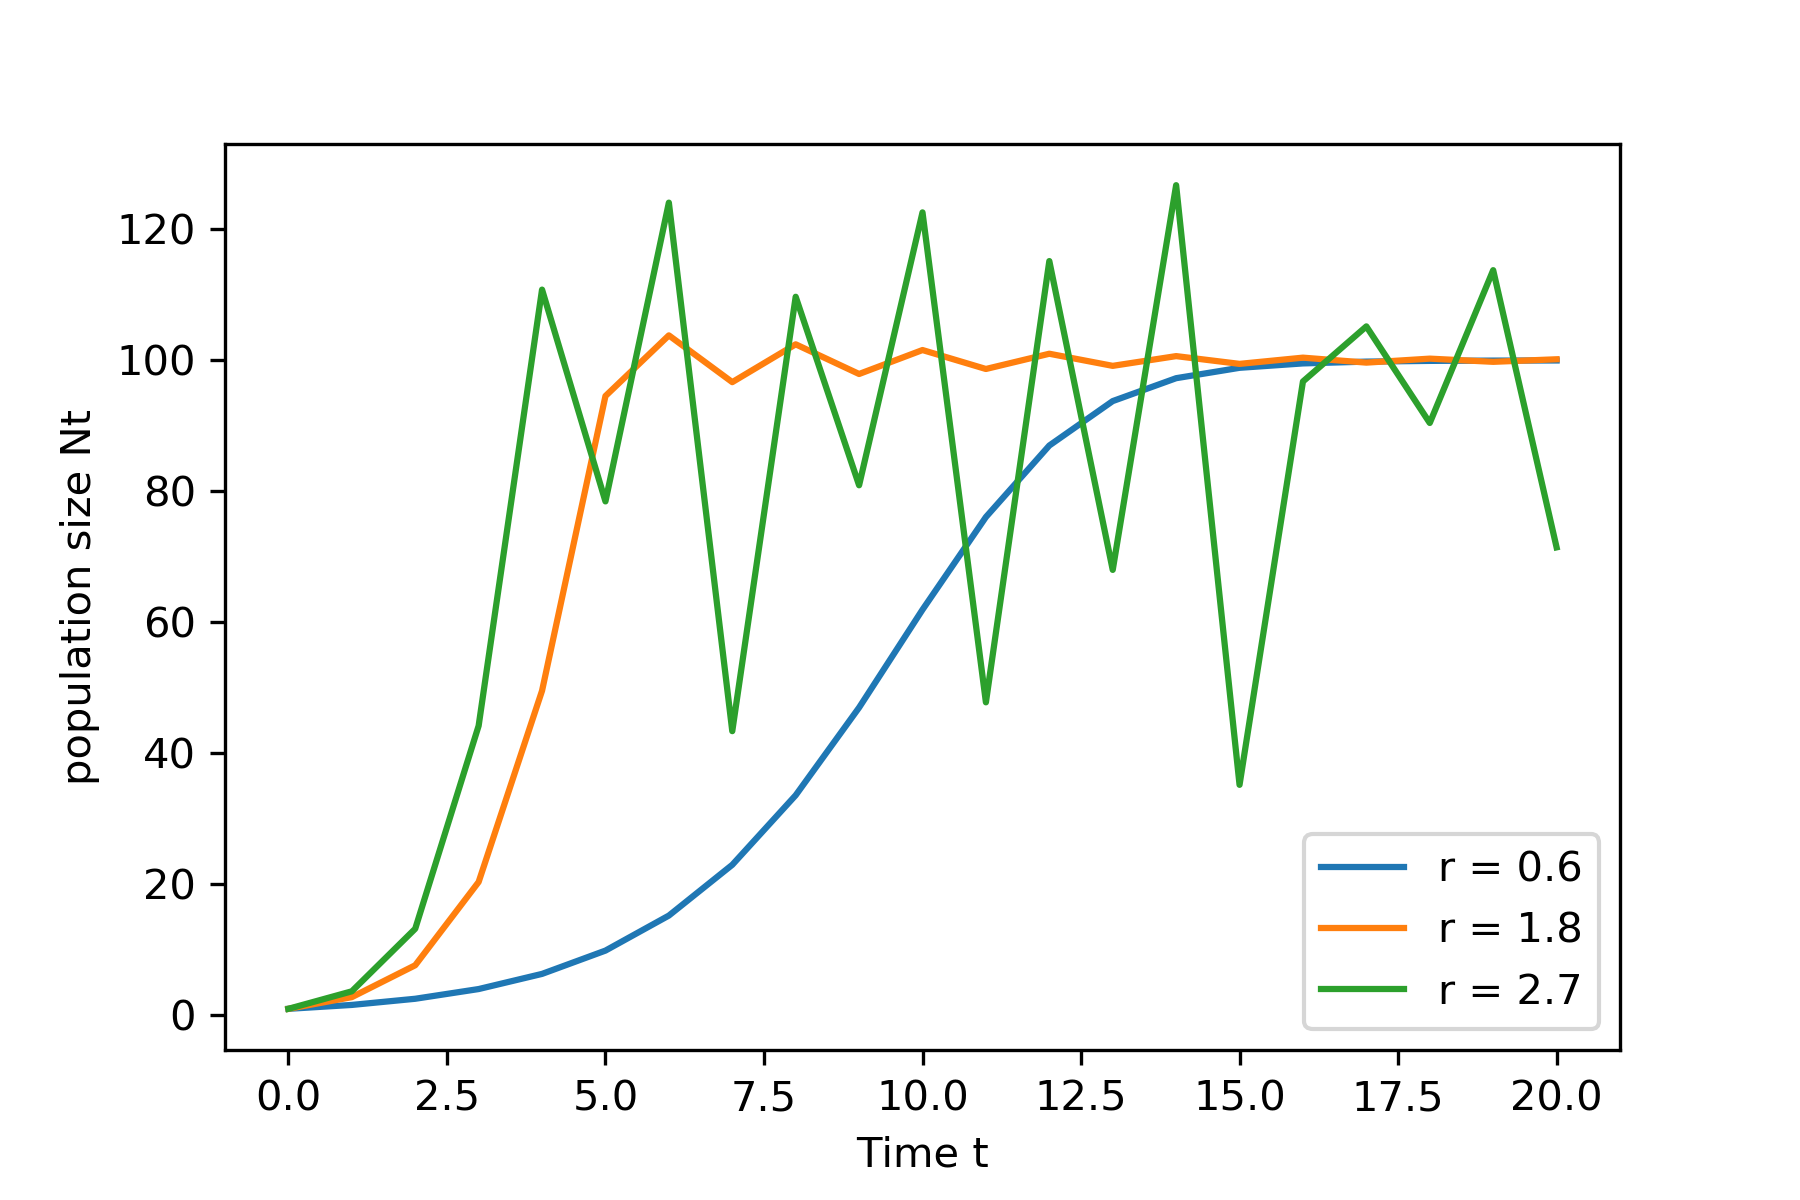
\includegraphics[width=0.8\linewidth]{hw1.png}
	\caption{図2 r値による各挙動の}
	\end{figure}
	\newpage
\subsection*{練習2}
	収束値のプロットによる分岐図を以下の図3に示す.なお実行したプログラムファイルは0418-2.pyである.
	\begin{figure}[H]
	\centering
	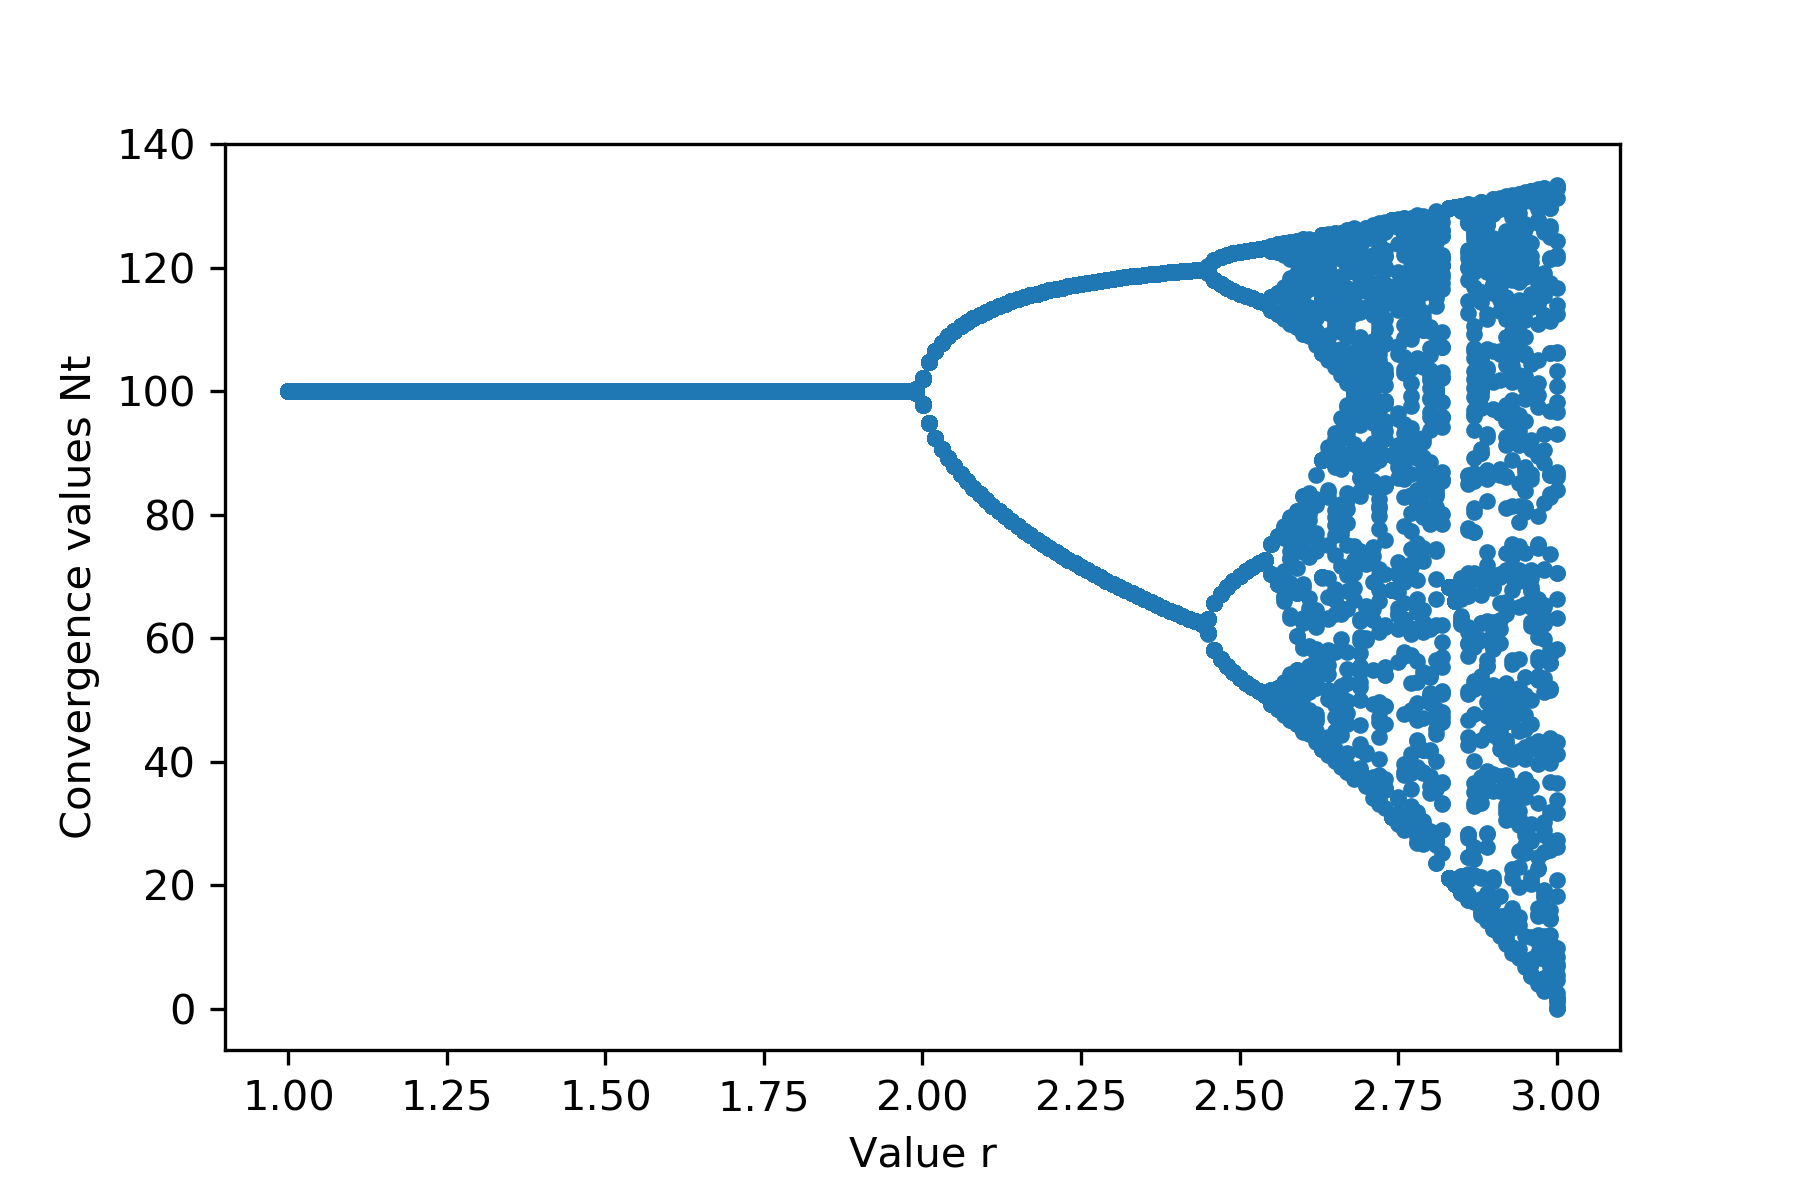
\includegraphics[width=0.8\linewidth]{hw2.png}
	\caption{図3 分岐図}
	\end{figure}


\end{document}
